\section{支持向量机}
在logistic回归中,概率$p(y=1|x;\theta)$由$h_\theta(x)=g(\theta^Tx)$得出。当$h_\theta(x)\geq 0.5$时认为预测值为1,而这种情况对应的是$\theta^Tx\geq0$。当$\theta_Tx$越大,则$p(y=1|x;\theta,b)$则越大,可以认为更加确信预测值是1。因此当有$\theta^Tx\gg0$,认为$y=1$的结果是非常有信心的;相反当有$\theta^Tx\ll0$,认为$y=0$的结果是非常有信心的。因而对于一个训练集,我们或许可以找到一个好的模型,即找到$\theta$,使当$y^{(i)}=1$时,有$\theta^Tx^{(i)}\gg0$,当$y^{(i)}=0$时,有$\theta^Tx^{(i)}\ll0$。事实上,支持向量机(Support Vector Machine)就是采取上述的思想,找到一个分割平面,让训练集的数据点离平面尽可能远。
\subsection{说明}
首先考虑二分类问题,用$y\in\{-1,1\}$而不是$\{0,1\}$来表示类标签;区别于logistic回归中对于线性模型的表示$\theta^Tx$,采用参数$w,b$,则分类器如下
\begin{eqnarray}
h_{w,b}(x)=g(w^Tx+b)\\
g(z)=
\left\lbrace
\begin{aligned}
1&, z\geq 0\\
-1&, otherwise
\end{aligned}
\right.
\end{eqnarray}
在这里,$w,b$的表示法可以截距$b$和其他参数$w$区分出来。于此同时,我们也去掉了$x$中的$x_0=1$这个与$b$相配套的维度。
\subsection{函数间隔与几何间隔}
\subsubsection{函数间隔}
对给定的训练数据$(x^{(i)},y^{(i)})$,定义函数间隔
\begin{eqnarray}
\hat{\gamma}^{(i)}=y^{(i)}(w^Tx+b)
\end{eqnarray}
如果$y^{(i)}=1$,为了让数据点离平面够大,则可让$\hat{\gamma}^{(i)}$足够大,则可让$w^Tx+b\gg0$。相反的,如果$y^{(i)}=-1$,为了让数据点离平面够大,则可让$\hat{\gamma}^{(i)}$足够大,则可让$w^Tx+b\ll0$。因而,可以得到足够大的函数间隔,可以得到置信度高且正确的预测。

然而,函数间隔的一个属性,使得其不能作为一个好的指标来度量置信度(有多大的把握正确):对于给定的$g$,如果用$2w$和$2b$分别代替$w$和$b$,因为$g(w^Tx+b)=g(2w^Tx+2b)$,所以$h_{w,b}(x)=h_{2w,2b}(x)$,然而函数间隔已经改变:
\begin{eqnarray}
2y^{(i)}(w^Tx+b)=y^{(i)}(2w^Tx+2b)
\end{eqnarray}
因此若$w,b$没有限制,则可以让函数间隔任意大,但其实际是没有意义的。因而考虑引入一些像$||w||_2=1$的正则化条件,或者可以用$(\frac{w}{||w||_2},\frac{b}{||w||_2})$来替代原有的$(w,b)$。这些后面会有所提及。

对于给定的训练集$S=\{(x^{(i)},y^{(i)});i=1,\cdots,m\}$,定义训练集$S$的函数间隔为
\begin{eqnarray}
\hat{\gamma}=\min_{i=1,\cdots,m}\hat{\gamma}^{(i)}
\end{eqnarray}
\subsubsection{几何间隔}
考虑下图:
\begin{center}
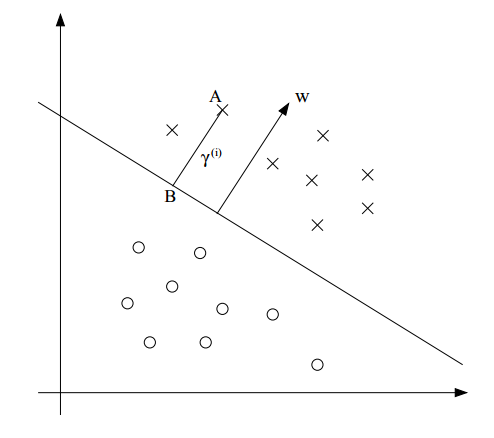
\includegraphics[scale=0.6]{../figures/SVM1.PNG} 
\end{center}
其中,实线为超平面$w^T+b$,向量$w$为超平面的法向量,则$\frac{w}{||w||_2}$位超平面的单位法向量。点$A$表示某个数据点,其所在位置代表输入向量$x^{(i)}$且其标签$y^{(i)}=1$,A到超平面距离为$\gamma^{(i)}$,其为$||AB||_2$。则有
\begin{eqnarray}
\overrightarrow{BA}=\frac{w}{||w||_2}\gamma^{(i)}
\end{eqnarray}
则
\begin{eqnarray}
B=x^{(i)}-\frac{w}{||w||_2}\gamma^{(i)}
\end{eqnarray}
由B在平面上,则有
\begin{eqnarray}
w^T\left( x^{(i)}-\frac{w}{||w||_2}\gamma^{(i)} \right)+b=0
\end{eqnarray}
则可以解出
\begin{eqnarray}
\begin{aligned}
\gamma^{(i)}&=\frac{w^Tx^{(i)}+b}{||w||_2}\\
&=\left(\frac{w}{||w||_2}\right)x^{(i)}+\frac{b}{||w||_2}
\end{aligned}
\end{eqnarray}
因而对于训练集中的数据$(x^{(i)},y^{(i)})$,定义几何间隔
\begin{eqnarray}
\gamma^{(i)}=y^{(i)}
\left(
\left(\frac{w}{||w||_2}
\right)^Tx^{(i)}+\frac{b}{||w||_2}
\right)
\end{eqnarray}
可见,当$||w||_2=1$时,函数间隔等于几何间隔。当用$2w$和$2b$分别代替$w$和$b$时,由于分母$||w||_2$的作用,使得
\begin{eqnarray}
y^{(i)}
\left(
\left(\frac{w}{||w||_2}
\right)^Tx^{(i)}+\frac{b}{||w||_2}
\right)
=
y^{(i)}
\left(
\left(\frac{2w}{||2w||_2}
\right)^Tx^{(i)}+\frac{2b}{||2w||_2}
\right)
\end{eqnarray}
几何间隔保持不变。因而可以对$w,b$进行任意的缩放,让其具有一些独特性质。

对于给定的训练集$S=\{(x^{(i)},y^{(i)});i=1,\cdots,m\}$,定义训练集$S$的几何间隔为
\begin{eqnarray}
\gamma=\min_{i=1,\cdots,m}\gamma^{(i)}
\end{eqnarray}

\subsection{最优间隔分类器}
根据上述方法,为了找到一个超平面将训练集分类,且训练集到超平面的几何间隔最大,有如下公式
\begin{eqnarray}
\begin{aligned}
\max_{\gamma,w,b}\gamma\\
s.t. & \sample{y}{i}(w^T\sample{x}{i}+b)\geq \gamma,i=1,\cdots,m\\
& ||w||=1
\end{aligned}
\end{eqnarray}
对于上述优化问题,由于$||w||=1$非凸,难以用最优化软件求解,因而尝试变型
\begin{eqnarray}
\begin{aligned}
\max_{\gamma,w,b}\frac{\hat{\gamma}}{||w||}\\
s.t. & \sample{y}{i}(w^T\sample{x}{i}+b)\geq \gamma,i=1,\cdots,m\
\end{aligned}
\end{eqnarray}
由于$\frac{\hat{\gamma}}{||w||}$非凸,需要进一步变型。考虑到可以对$w,b$进行缩放,使得$\hat{\gamma}=1$,又求解$\frac{\hat{\gamma}}{||w||}=\frac{\hat{1}}{||w||}$的最大值等价于求解$\frac{1}{2}||w||^2$的最小值,则有
\begin{eqnarray}
\begin{aligned}
\min_{\gamma,w,b} &\ \frac{1}{2}||w||^2\\
s.t. &\ \sample{y}{i}(w^T\sample{x}{i}+b)\geq 1,i=1,\cdots,m\
\end{aligned}
\end{eqnarray}
此时,这个形式的优化问题可以高效求解,其包含凸二次项和线性约束项,这给出了最有间隔分类器。

\subsection{约束优化问题}
\subsubsection{等式约束优化问题}
考虑以下的问题
\begin{eqnarray}
\begin{aligned}
\min_w &\ f(w)\\
s.t. &\ h_i(w)=0,i=1,\cdots,l
\end{aligned}
\end{eqnarray}
定义拉格朗日算子(Lagrangian)如下
\begin{eqnarray}
\mathcal{L}(w,\beta)=f(w)+\sum_{i=1}^l\beta_ih_i(w)
\end{eqnarray}
其中,$\beta_i$称为拉格朗日乘子(Lagrange multipliers),对上式分别对$w_i$和$\beta_i$求偏导
\begin{eqnarray}
\frac{\partial\cal{L}}{\partial w_i}&=&0,i=1,2,\cdots,n\\
\frac{\partial\cal{L}}{\partial \beta_i}&=&0,i=1,2,\cdots,l\\
\end{eqnarray}
从而求解q$w$和$\beta$。得到的解可能极值点,此方程组称为等式约束的极值必要条件。此方法相当于将拉格朗日乘子$\beta_i$和$x_i$一起看为优化变量,则优化变量个数增加为$n+l$个。$\beta_i$和$x_i$一视同仁,均为优化变量,均对他们求偏导。

\subsubsection{不等式约束优化问题}
考虑一个一元函数的例子
\begin{eqnarray}
\begin{aligned}
\min &\ f(x)\\
s.t. &\ g_1(x)=a-x\leq 0\\
&\ g_2(x)=x-b\leq 0
\end{aligned}
\end{eqnarray}

对于约束$g_1$和$g_2$,我们分别引入两个松弛变量$a_1^2$和$b_1^2$,得到$$h_1(x,a_1)=g_1+a_1^2=0$和$h_2(x,b_1)=g_2+b_1^2=0$,此处考虑加上平方项$a_1^2,b_1^2$而不是$a_1,b_1$,因为其能隐含的反映其大于等于0的性质。若只加上$a_1$和$b_1$,则需要引入新的约束$a_1\geq 0$和$b_1\geq 0$,这会让问题复杂化。于是,我们将不等式约束转化为了等式约束
\begin{eqnarray}
\begin{aligned}
\min &\ f(x)\\
s.t. &\ h_1(x,a_1)=g_1+a_1^2=a-x+a_1^2=0\\
&\ h_2(x,b_1)=g_2+b_1^2=x-b+b_1^2=0
\end{aligned}
\end{eqnarray}
于是可以得到拉格朗日函数
\begin{eqnarray}
\mathcal{L}(x,a_1,b_1,\mu_1,\mu_2)=f(x)+\mu_1(a-x+a_1^2)+\mu_2(x-b+b_1^2)
\end{eqnarray}
对各变量求偏导,联立方程,有
\begin{eqnarray}
\left\lbrace
\begin{aligned}
\frac{\partial \mathcal{L}}{\partial x}=\frac{\partial f}{\partial x}+\mu_1\frac{dg_1}{dx}+\mu_2\frac{dg_2}{dx}=\frac{df}{dx}-\mu_1+\mu_2=0,\\
\frac{\partial \mathcal{L}}{\partial \mu_1}=g_1+a_1^2=0,\ \frac{\partial \mathcal{L}}{\partial \mu_2}=g_2+b_1^2=0,\\
\frac{\partial \mathcal{L}}{\partial a_1}=2\mu_1a_1=0,\ 
\frac{\partial \mathcal{L}}{\partial b_1}=2\mu_2b_1=0,\\
\mu_1\geq 0,\ \mu_2\geq 0
\end{aligned}
\right.
\end{eqnarray}
其可转化为
\begin{eqnarray}
\left\lbrace
\begin{aligned}
\frac{\partial f}{\partial x}+\mu_1\frac{dg_1}{dx}+\mu_2\frac{dg_2}{dx}=0,\\
\mu_1g_1=0,\ \mu_2g_2=0,\\
\mu_1\geq 0,\ \mu_2\geq 0
\end{aligned}
\right.
\end{eqnarray}
对于多元多次不等式约束问题
\begin{eqnarray}
\begin{aligned}
\min_w &\ f(x)\\
s.t.&\  g_j(x)\leq0(j=1,2,\cdots,m)
\end{aligned}
\end{eqnarray}
有
\begin{eqnarray}
\left\lbrace
\begin{aligned}
\frac{\partial f(x^*)}{\partial x_i}+\sum_{j=1}^m\mu_j\frac{\partial g_j(x^*)}{\partial x_i}=0, i=1,2\cdots,n,\\
\mu_jg_j(x^*)=0, j=1,2,\cdots,m,\\
\mu_j\geq 0,j=1,2,\cdots,m
\end{aligned}
\right.
\end{eqnarray}
上式称为不等式约束优化问题的KKT(Karush-Kuhn-Tucker)条件,$\mu_j$称为KKT乘子。当约束起作用时$\mu_j> 0,g_j(x)=0$,约束不起作用时有$\mu_j= 0,g_j(x)<0$。\footnote{参考自https://zhuanlan.zhihu.com/p/26514613}

让其与CS229采用同样的记法,对于原问题
\begin{eqnarray}
\begin{aligned}
\min_w &\ f(w)\\
s.t. &\ g_i(w)\leq0,i=1,\cdots,k\\
&\ h_i(w)=0,i=1,\cdots,l
\end{aligned}
\end{eqnarray}
拉格朗日函数为
\begin{eqnarray}
\mathcal{L}(w,\alpha,\beta)=f(w)+\sum_{i=1}^k\alpha_ig_i(w)+\sum_{i=1}^l\beta_ih_i(w)
\end{eqnarray}
考虑量
\begin{eqnarray}
\theta_p(w)&=&\max_{\alpha,\beta:\alpha\geq0}\mathcal{L}(w,\alpha,\beta)\\
&=&\max_{\alpha,\beta:\alpha\geq0}\ f(w)+\sum_{i=1}^k\alpha_ig_i(w)+\sum_{i=1}^l\beta_ih_i(w)
\end{eqnarray}
定义原问题的最优值为
\begin{eqnarray}
p^*=\min_w\theta_p(w)
\end{eqnarray}
另一方面,考虑对偶问题,可得到
\begin{eqnarray}
\theta_D(\alpha,\beta)=\min_w\mathcal{L}(w,\alpha,\beta)
\end{eqnarray}
定义对偶问题的最优值为
\begin{eqnarray}
d^*=\max_{\alpha,\beta:\beta_i\geq0}\theta_D(w)
\end{eqnarray}
原问题和对偶问题的关系为
\begin{eqnarray}
d^*=\max_{\alpha,\beta:\beta_i\geq0}\min_w\mathcal{L}(w,\alpha,\beta)\leq \min_w\max_{\alpha,\beta:\beta_i\geq0}\mathcal{L}(w,\alpha,\beta)=p^*
\end{eqnarray}
当
\begin{eqnarray}
d^*=p^*
\end{eqnarray}
时,为强对偶,此时,原问题和对偶问题会取相同的值。\\

所得的KKT条件为
\begin{eqnarray}
\frac{\partial}{\partial w_i}\mathcal{L}(w^*,\alpha^*,\beta^*)&=&0,i=1,\cdots,n\\
\frac{\partial}{\partial \beta_i}\mathcal{L}(w^*,\alpha^*,\beta^*)&=&0,i=1,\cdots,l\\
\alpha_i^*g_i(w^*)&=&0,i=1,\cdots,k\\
g_i(w^*)&\leq&0,i=1,\cdots,k\\
\alpha^*&\geq& 0,i=1,\cdots,k
\end{eqnarray}
如果$w^*,\alpha^*,\beta^*$满足KKT条件,则其为原问题和对偶问题的一个解。其中,$\alpha_i^*g_i(w^*)=0,i=1,\cdots,k$被称为KKT对偶互补条件( KKT dual complementarity condition),它表明如果$\alpha_i^*>0$,则$g_i(w^*)=0$
\subsection{最优间隔分类器的求解}
对之前,已得到
\begin{eqnarray}
\begin{aligned}
\min_{\gamma,w,b} &\ \frac{1}{2}||w||^2\\
s.t. &\ \sample{y}{i}(w^T\sample{x}{i}+b)\geq 1,i=1,\cdots,m\
\end{aligned}
\end{eqnarray}
可将约束写成
\begin{eqnarray}
g_i(w)=-\sample{y}{i}(w^T\sample{x}{i}+b)+1\leq 0,
\end{eqnarray}
从KKT对偶互补条件可知,当训练数据点的函数间隔等于1时,才会有$\alpha_i>0$
其拉格朗日函数为
\begin{eqnarray}
\mathcal{L}(w,b,\alpha)=\frac{1}{2}||w||^2-\sum_{i=1}^m\alpha_i\sample{y}{i}(w^T\sample{x}{i}+b)-1]
\end{eqnarray}
其中,$\alpha_i$为KKT乘子,而不需要$\beta_i$拉格朗日乘子,因为该问题中只有不等式约束。

考虑下图:

\begin{center}
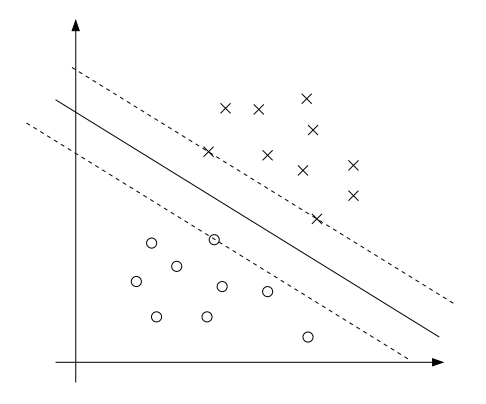
\includegraphics[scale=0.6]{../figures/SVM2.PNG} 
\end{center}
其中,实线表示最大间隔平面。图中,有三个点的间隔最小,有一个是负类,两个是正类,它们位于与超平面平行的虚线上。因此,这三个数据点所对应的$\alpha_i$非0,我们称这三个数据点为该问题的支持向量(support vectors)。事实上,支持向量的数目会比训练集中的数据数目少很多。

解对偶问题,首先固定$\alpha$,对$\mathcal{L}(w,b,\alpha)$,分别求$w,b$的偏导,令偏导数等于0,有
\begin{eqnarray}
\nabla_w\mathcal{L}(w,b,\alpha)=w-\sum_{i=1}^m\alpha_i\sample{y}{i}\sample{x}{i}&=&0\\
\frac{\partial}{\partial b}\mathcal{L}(w,b,\alpha)&=&0
\end{eqnarray}
得
\begin{eqnarray}
w&=&\sum_{i=1}^m\alpha_i\sample{y}{i}\sample{x}{i}\\
\sum_{i=1}^m\alpha_i\sample{y}{i}&=&0
\end{eqnarray}
代入则有
\begin{eqnarray}
\begin{aligned}
\mathcal{L}(w,b,\alpha)&=\frac{1}{2}w^Tw-\sum_{i=1}^m\alpha_i(\sample{y}{i}(w^T\sample{x}{i}+b)-1)\\
&=\frac{1}{2}\left(\sum_{i=1}^m \alpha_i\sample{y}{i}\sample{x}{i}\right)^T\left(\sum_{i=j}^m \alpha_j\sample{y}{j}\sample{x}{j}\right)-
\sum_{i=1}^m\alpha_i
	( 
	\sample{y}{i} 
		(
			(
				\left(\sum_{i=j}^m \alpha_j\sample{y}{j}\sample{x}{j}\right)^T\sample{x}{i}+b
			)-1
		) 
	)\\
&=\frac{1}{2}\sum_{i=1}^m\sum_{j=1}^m\sample{y}{i}\sample{y}{j}\alpha_i\alpha_j\langle\sample{x}{i},\sample{x}{j}\rangle-\sum_{i=1}^m\sum_{j=1}^m\sample{y}{i}\sample{y}{j}\alpha_i\alpha_j\langle\sample{x}{i},\sample{x}{j}\rangle+\sum_{i=1}^m\alpha_i\\
&=\sum_{i=1}^m\alpha_i-\frac{1}{2}\sum_{i=1}^m\sum_{j=1}^m\sample{y}{i}\sample{y}{j}\alpha_i\alpha_j\langle\sample{x}{i},\sample{x}{j}\rangle-b\sum_{i=1}^m\alpha_i\sample{y}{i}\\
&=\sum_{i=1}^m\alpha_i-\frac{1}{2}\sum_{i=1}^m\sum_{j=1}^m\sample{y}{i}\sample{y}{j}\alpha_i\alpha_j\langle\sample{x}{i},\sample{x}{j}\rangle
\end{aligned}
\end{eqnarray}
其中,$\langle\sample{x}{i},\sample{x}{j}\rangle=(\sample{x}{i})^T\sample{x}{j}$,令
\begin{eqnarray}
W(\alpha)=\sum_{i=1}^m\alpha_i-\frac{1}{2}\sum_{i=1}^m\sum_{j=1}^m\sample{y}{i}\sample{y}{j}\alpha_i\alpha_j\langle\sample{x}{i},\sample{x}{j}\rangle
\end{eqnarray}
我们可以得到如下的原问题的对偶问题
\begin{eqnarray}
\begin{aligned}
\max_\alpha&\ W(\alpha)=\sum_{i=1}^m\alpha_i-\frac{1}{2}\sum_{i=1}^m\sum_{j=1}^m\sample{y}{i}\sample{y}{j}\alpha_i\alpha_j\langle\sample{x}{i},\sample{x}{j}\rangle\\
s.t.&\ \alpha_i\geq 0,i=1,2,\cdots,m\\
&\ \sum_{i=1}^m\alpha_i\sample{y}{i}=0
\end{aligned}
\end{eqnarray}
其符合KKT条件,因而可以求解$\alpha$,通过$w=\sum_{i=1}^m\alpha_i\sample{y}{i}\sample{x}{i}$求解$w$,对于$b$的求解,考虑到可以用离超平面最相近的两类点的中点来求$b$。设上面求得的$w$为$w^*$,则有
\begin{eqnarray}
b^*=-\frac{\max_{i:\sample{y}{i}=-1}w^{*T}\sample{x}{i}+\min_{i:\sample{y}{i}=1}w^{*T}\sample{x}{i}}{2}
\end{eqnarray}

\subsection{核方法}
定义原始输入值为某个问题的输入属性(input attributes),由输入属性延伸出来的新变量定义为输入特征(input features),用$\phi$表示特征映射,比如如下的将输入属性映射为输入特征的函数
\begin{eqnarray}
\phi(x)=
\begin{pmatrix}
x\\
x^2\\
x^3
\end{pmatrix}
\end{eqnarray}

由于我们可以得到的最优间隔分类器为如下形式
\begin{eqnarray}
\begin{aligned}
\max_\alpha&\ W(\alpha)=\sum_{i=1}^m\alpha_i-\frac{1}{2}\sum_{i=1}^m\sum_{j=1}^m\sample{y}{i}\sample{y}{j}\alpha_i\alpha_j\langle\sample{x}{i},\sample{x}{j}\rangle\\
s.t.&\ \alpha_i\geq 0,i=1,2,\cdots,m\\
&\ \sum_{i=1}^m\alpha_i\sample{y}{i}=0
\end{aligned}
\end{eqnarray}
对于算法中所含有$\langle x,z\rangle$,我们可以将其替换为$\langle\phi(x),\phi(z)\rangle$。另外,对于给定的特征映射$\phi$,定义其对应的核(kernel)为
\begin{eqnarray}
K(x,z)=\phi(x)^T\phi(z)
\end{eqnarray}
因此,对于算法中含有的$\langle x,z\rangle$,我们可以替换为$K(x,z)$,此时算法就可以基于特征函数$\phi$来学习。

对于给定的$\phi$,我们可以通过计算$\phi(x)$和$\phi(z)$以及计算其内积来很容易地得到$K(x,z)$。虽然$K(x,z)$计算的代价不高,但$\phi(x)$计算代价可能会很高(可能因为它是一个非常高维的向量)。在这种设置下,我们让SVMs在更高维度中学习(对于给定的$\phi$),而不需要显式地调用向量$\phi(x)$

考察土哥例子。对于$x,z\in \mathbb{R}^n$,考虑
\begin{eqnarray}
\begin{aligned}
K(x,z)&=(x^Tz)^2\\
&= \left(\sum_{i=1}^nx_iz_i\right)\left(\sum_{j=1}^nx_jz_j\right)\\
&= \sum_{i=1}^n\sum_{j=1}^nx_ix_jz_iz_j\\
&= \sum_{i=1}^n\sum_{j=1}^n(x_ix_j)(z_iz_j)
\end{aligned}
\end{eqnarray}
因此,$K(x,z)=\phi(x)^T\phi(z)$,其中特征映射$\phi$为如下形式(只给出$n=3$时的情况)
\begin{eqnarray}
\phi(x)=
\begin{pmatrix}
x_1x_1\\
x_1x_2\\
x_1x_3\\
x_2x_1\\
x_2x_2\\
x_2x_3\\
x_3x_1\\
x_3x_2\\
x_3x_3
\end{pmatrix}
\end{eqnarray}
这种情况下,计算高维的$\phi(x)$需要$O(n^2)$的时间,而$K(x,z)$只需要$O(n)$的时间。

作为一个相似的核,考虑
\begin{eqnarray}
\begin{aligned}
K(x,z)&=(x^Tz+c)^2\\
&=\left(\sum_{i=1}^nx_iz_i+c\right)\left(\sum_{j=1}^nx_jz_j+c\right)\\
&=\sum_{i=1}^n\sum_{j=1}^n(x_ix_j)(z_iz_j)+2c\sum_{i=1}^nx_iz_i+c^2\\
&=\sum_{i=1}^n\sum_{j=1}^n(x_ix_j)(z_iz_j)+\sum_{i=1}^n(\sqrt{2c}x_i)(\sqrt{2c}z_i)+c^2
\end{aligned}
\end{eqnarray}
则其相应的特征映射为
\begin{eqnarray}
\phi(x)=
\begin{pmatrix}
x_1x_1\\
x_1x_2\\
x_1x_3\\
x_2x_1\\
x_2x_2\\
x_2x_3\\
x_3x_1\\
x_3x_2\\
x_3x_3\\
\sqrt{2c}x_1\\
\sqrt{2c}x_2\\
\sqrt{2c}x_3\\
c
\end{pmatrix}
\end{eqnarray}
其中,参数$c$用来控制$x_i$和$x_ix_j$的权重。

更一般的,核$K(x,z)=(x^Tz+c)^d$对应一个特征映射(映射到$\left(_d^{n+d}\right)$的特征空间)。虽然是在$O(n^d)$维空间中计算,但是计算$K(x,z)$依然只需要$O(n)$的时间,因此,我们不需要显式地在很高维的特征空间中表示特征向量。

接下来,考察一种略微不同的核。直观地,若$\phi(x)$和$\phi(z)$非常接近,则我们希望$K(x,z)=\phi(x)T\phi(z)$是大的。相反的,若$\phi(x)$和$\phi(z)$距离很远(假设已经接近彼此正交),则我们希望$K(x,z)=\phi(x)T\phi(z)$是小的。因此设想$K(x,z)$是一种度量规则,来度量$\phi(x)$和$\phi(z)$有多接近,或者$x$和$z$有多接近。

\subsubsection{高斯核函数}
直觉上,可能会想到这样的一个函数
\begin{eqnarray}
K(x,z)=\exp\left(
-\frac{||x-z||^2}{2\sigma^2}
\right)
\end{eqnarray}
当$x$和$z$接近时,则该值趋近与1;当距离远时,该值趋近于0。它可以用作SVM的一个核。(这个核称为高斯核,对应于有限维特征映射$\phi$)。

\subsubsection{核的有效性}
作为问题的推广,对于给定的函数$K$,如何判断其是否是有效的核?比方说有这样的问题:是否存在特征映射$\phi$,使对于所有$x,z$,都有$K(x,z)=\phi(x)^T\phi(z)$?

假设$K$确实是一个对应于某个特征映射$\phi$的有效的核,那么考虑有限的$m$个点的集合$\{\sample{x}{1},\cdots,\sample{x}{m}\}$,定义一个$m\times m$的方阵$K$,其中$K_{ij}=K(\sample{x}{i},\sample{x}{j})$,并将$K$称为核矩阵(Kernel matrix)。

若$K$是一个有效的核,则
\begin{eqnarray}
\begin{aligned}
K_{ij} &= K(\sample{x}{i},\sample{x}{j})\\
&= \phi(\sample{x}{i})^T\phi(\sample{x}{j})\\
&= \phi(\sample{x}{j})^T\phi(\sample{x}{i})\\
&= K(\sample{x}{j},\sample{x}{i})\\
&= K_{ji}
\end{aligned}
\end{eqnarray}
因此,$K$必须是对称的。定义$\phi_k(x)$为向量$\phi(x)$的第$k$个维度,则对于任意的向量$z$,我们有
\begin{eqnarray}
\begin{aligned}
z^TKz&=\vectornew{z}{m}\matrixthird{K}{m}{m}\vvectornew{z}{m}\\
&= \left(\sum_{i=1}^mZ_iK_{i1},\sum_{i=1}^mZ_iK_{i2},\cdots,\sum_{i=1}^mZ_iK_{im}\right)\vvectornew{z}{m}\\
&= \sum_i^m\sum_j^mz_iK_{ij}z_j\\
&= \sum_i^m\sum_j^mz_i\phi(\sample{x}{i})^T\phi(\sample{x}{j})z_j\\
&= \sum_i^m\sum_j^mz_i\sum_k^m\phi_k(\sample{x}{i})\phi_k(\sample{x}{j})z_j\\
&= \sum_k^m\sum_i^m\sum_j^mz_i\phi_k(\sample{x}{i})\phi_k(\sample{x}{j})z_j\\
&= \sum_k^m\left(\sum_{i=1}z_i\phi_k(\sample{x}{i})\right)\\
&\geq 0
\end{aligned}
\end{eqnarray}
由于$z^TKz\geq 0$,且$z$是任意的,因为$K$是半正定矩阵($K\geq 0$)。

因此,如果$K$是一个有效的核(设其对应于特征映射$\phi$),那么其对应的核矩阵$K\in \mathbb{R}^{m\times m}$是半正定的。这是充分非必要的。这个有效的核称为Mercer kernel。

\paragraph{Mercer 定理} $K$是$\mathbb{R}^n\times\mathbb{R}^n\mapsto\mathbb{R}$的映射,$K$是有效的(kercer)核的充分必要条件为对于任意$\{\sample{x}{1},\cdots,\sample{x}{m}\}$,$m<\infty$,其对应的核矩阵是半正定的。

其中,任意$\{\sample{x}{1},\cdots,\sample{x}{m}\}$是任意一个包含有$m$个样本的集合,并不一定是训练集,可以任选。

对于给定的函数$K$,除了尝试找到一个对应于$K$的特征映射$\phi$,该理论给出了另一种方法去测试$K$是否是一个有效核。


\subsection{正则化和非线性可分情况}
到目前SVM假设数据是线性可分的。因为通过$\phi$将数据映射到高维的特征空可以提高数据可分的可能性,但是我们不能保证一直可以达到这种效果。而且有的时候我们也不必赢定要去寻找这个超平面,由于一些异常点。举个例子,左边表示了一个最优的间隔分类器,但当一个异常点加入到了左边的数据点之后,导致判平面发生了戏剧性的旋转,而且其产生的分类器只有一个很小的间隔。
\begin{center}
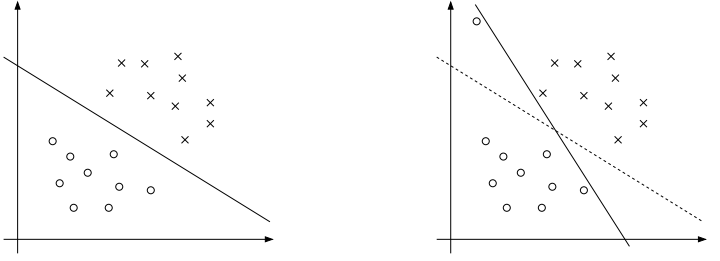
\includegraphics[scale=0.6]{../figures/SVM3.PNG} 
\end{center}

为了让算法适用于非线性可分的数据,同时降低对于异常点的灵敏性,我们重新修改了最优化分类器,其结果如下
\begin{eqnarray}
\begin{aligned}
\min_{\gamma,w,b}&\ \frac{1}{2}||w||^2+C\sum_{i=1}^m\xi_i\\
s.t.&\ \sample{y}{i}(w^T\sample{x}{i}+b)\geq 1-\xi_i,i=1,\cdots,m\\
&\ \xi_i\geq 0,i=1,\cdots,m
\end{aligned}
\end{eqnarray}
因此,这种改进可以允许函数间隔小于1,若有某个例子的函数间隔为$1-\xi_i$,它将会在目标函数上付出$C\xi_i$的代价。参数$C$用来权衡要让$||w||^2$大(将会让函数间隔变小)还是尽量保证大部分的数据能够有函数间隔至少等于1。

就像之前的,我们可以得到拉格朗日函数如下
\begin{eqnarray}
\mathcal{L}(w,b,\xi,\alpha,r)=\frac{1}{2}||w||^2+C\sum_{i=1}^m\xi_i-\sum_{i=1}^m\alpha_i[\sample{y}{i}(w^T\sample{x}{i}+b)-1+\xi_i]-\sum_{i=1}^mr_i\xi_i
\end{eqnarray}

其中,$\alpha_i$和$r_i$是KKT乘子。分别对$w,b,\xi$求偏导,有
\begin{eqnarray}
\nabla_w\mathcal{L}=w-\sum_{i=1}^m\alpha_i\sample{y}{i}\sample{x}{i}=0\\
\nabla_n\mathcal{L}=-\sum_{i=1}^m\alpha_i\sample{y}{i}=0\\
\nabla_{\xi_i}\mathcal{L}=C-\alpha_i-r_i=0,i=1,2,\cdots,m
\end{eqnarray}

\begin{eqnarray}
\begin{aligned}
\mathcal{L}(w,b,\xi,\alpha,r)&=\frac{1}{2}||w||^2+C\sum_{i=1}^m\xi_i-\sum_{i=1}^m\alpha_i[\sample{y}{i}(w^T\sample{x}{i}+b)-1+\xi_i]-\sum_{i=1}^mr_i\xi_i\\
&=\frac{1}{2}w^Tw+C\sum_{i=1}^m\xi_i-\sum_{i=1}^m\alpha_i[\sample{y}{i}(w^T\sample{x}{i}+b)-1+\xi_i]-\sum_{i=1}^mr_i\xi_i\\
&=\frac{1}{2}w^Tw-\sum_{i=1}^m\alpha_i[\sample{y}{i}(w^T\sample{x}{i}+b)-1]+C\sum_{i=1}^m\xi_i-\sum_{i=1}^m\alpha_i\xi_i-\sum_{i=1}^mr_i\xi_i\\
&=\frac{1}{2}w^Tw-\sum_{i=1}^m\alpha_i[\sample{y}{i}(w^T\sample{x}{i}+b)-1]+
\begin{pmatrix}
C\\
C\\
\vdots\\
C
\end{pmatrix}^T\vvectornew{\xi}{m}-\vvectornew{\alpha}{m}^T\vvectornew{\xi}{m}-\vvectornew{r}{m}^T\vvectornew{\xi}{m}\\
&=\frac{1}{2}w^Tw-\sum_{i=1}^m\alpha_i[\sample{y}{i}(w^T\sample{x}{i}+b)-1]+
\begin{pmatrix}
C-\alpha_1-r_1\\
C-\alpha_2-r_2\\
\vdots\\
C-\alpha_m-r_m
\end{pmatrix}^T\vvectornew{\xi}{m}\\
&=\frac{1}{2}w^Tw-\sum_{i=1}^m\alpha_i[\sample{y}{i}(w^T\sample{x}{i}+b)-1]\\
&=\sum_{i=1}^m\alpha_i-\frac{1}{2}\sum_{i=1}^m\sum_{j=1}^m\sample{y}{i}\sample{y}{j}\alpha_i\alpha_j\langle\sample{x}{i},\sample{x}{j}\rangle
\end{aligned}
\end{eqnarray}

我们可以得到如下的原问题的对偶问题
\begin{eqnarray}
\begin{aligned}
\max_\alpha&\ W(\alpha)=\sum_{i=1}^m\alpha_i-\frac{1}{2}\sum_{i=1}^m\sum_{j=1}^m\sample{y}{i}\sample{y}{j}\alpha_i\alpha_j\langle\sample{x}{i},\sample{x}{j}\rangle\\
s.t.&\ 0\leq \alpha_i \leq C,i=1,2,\cdots,m\\
&\ \sum_{i=1}^m\alpha_i\sample{y}{i}=0
\end{aligned}
\end{eqnarray}

就像之前一样,$w$依旧可以通过$\alpha$表示。让我们震惊的是,增加了$\mathcal{l}_1$正则项,对偶问题的改变只是在原有基础上由$0\leq\alpha_i$变为$0\leq\alpha_i\leq C$,$b^*$的求解也与之前一样。

同样的,KKT对偶互补条件(这些将在SMO算法中用到)如下
\begin{eqnarray}
\alpha_i=0 \Rightarrow \sample{y}{i}(w^T\sample{x}{i}+b)\geq 1\\
\alpha_i=C \Rightarrow \sample{y}{i}(w^T\sample{x}{i}+b)\leq 1\\
0<\alpha_i<C \Rightarrow \sample{y}{i}(w^T\sample{x}{i}+b)=1
\end{eqnarray}

\subsection{SMO算法}
SMO算法( sequential minimal optimization algorithm)给出一种有效率的方法来解决SVM所引出的对偶问题。首先考虑坐标提升算法(coordinate ascent algorithm)。

\subsubsection{坐标提升}
考虑解决一个无约束最优化问题
\begin{eqnarray}
\max_\alpha\ W\vectornew{\alpha}{m}
\end{eqnarray}
这里,我们认为$W$是一个关于$\alpha_i$的函数,而且我们先忽略任何该问题与SVMs的关系。接下来我们要探讨一个新的优化算法,称为梯度提升法:

\begin{center}
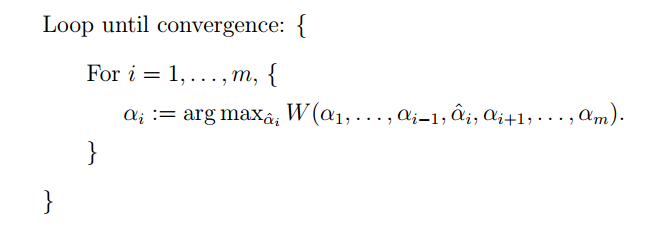
\includegraphics[scale=1]{../figures/SVM4.PNG} 
\end{center}

在算法的最里层循环中,我们让除了$\alpha_i$以外的变量保持固定,然后通过调整参数$\alpha_i$来反复优化$W$。在该算法的表示中,里层循环根据次序$\alpha_1,\alpha_2,\cdots,\alpha_m,\alpha_1,\alpha_2,\cdots$来反复优化变量。(其他更加复杂的版本可能会选择其他的次序,比如,我们可能会选择能够最大增长$W(\alpha)$的变量来优化。)

当函数$W$采取$\arg\max$的方式,则坐标提升将很有效率。下图为坐标提升的图
\begin{center}
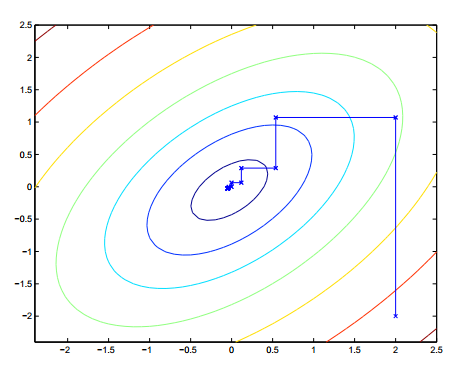
\includegraphics[scale=1]{../figures/SVM5.PNG} 
\end{center}

其中,椭圆表示我们要优化的二次函数的等高线。从坐标$(-2,2)$开始坐标提升,在图中画出其收敛到全局最大值的路径。可以注意到坐标提升每一步迭代都是平行于坐标轴,因一次为只有一个变量呗最优化。

\subsubsection{SMO}
下面的对偶优化问题我们将要求解的:
\begin{eqnarray}
\begin{aligned}
\max_\alpha&\ W(\alpha)=\sum_{i=1}^m\alpha_i-\frac{1}{2}\sum_{i=1}^m\sum_{j=1}^m\sample{y}{i}\sample{y}{j}\alpha_i\alpha_j\langle\sample{x}{i},\sample{x}{j}\rangle\\
s.t.&\ 0\leq \alpha_i \leq C,i=1,2,\cdots,m\\
&\ \sum_{i=1}^m\alpha_i\sample{y}{i}=0
\end{aligned}
\end{eqnarray}
假设我们有满足约束条件的$\alpha_i$的集合。现在,我们保持$\alpha_2,\cdots,\alpha_m$不变,然后用坐标提升的方法,通过优化$\alpha_1$来优化目标函数。但是这个方法是不可行的,因为约束条件有
\begin{eqnarray}
\alpha_1\sample{y}{1}=-\sum_{i=2}^m\alpha_i\sample{y}{i}
\end{eqnarray}
由于$\sample{y}{i}\in\{-1,1\}$,则有$(\sample{y}{1})^2=1$。对上式两边同时乘$\sample{y}{1}$,则可以得到
\begin{eqnarray}
\begin{aligned}
\alpha_1&=\alpha_1(\sample{y}{1})^2=-\sample{y}{1}\sum_{i=2}^m\alpha_i\sample{y}{i}
\end{aligned}
\end{eqnarray}
因此,$\alpha_1$由其他的$\alpha_i,i\neq1$确定。如果我们保持$\alpha_2,\cdots,\alpha_m$不变,则$\alpha_1$不能变,除非我们违背约束条件。因此,如果我们想要更新其中一些$\alpha$,则我们至少要同时改变两个以满足约束条件。于是其催生了SMO算法,其工作原理如下:
\begin{center}
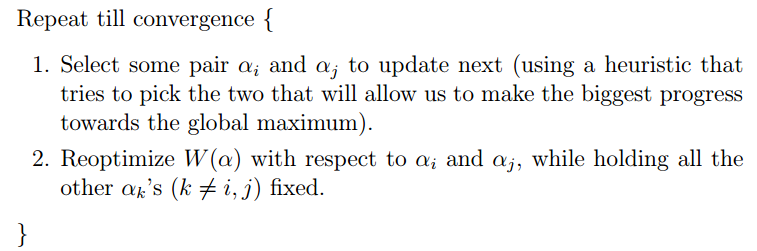
\includegraphics[scale=1]{../figures/SVM6.PNG} 
\end{center}
对于验证算法何时收敛,我们检验如下的KKT对偶互补条件是否在$tol$中,$tol$代表convergence tolerance parameter,其经常被设置在0.01到0.001。
\begin{eqnarray}
\alpha_i=0 \Rightarrow \sample{y}{i}(w^T\sample{x}{i}+b)\geq 1\\
\alpha_i=C \Rightarrow \sample{y}{i}(w^T\sample{x}{i}+b)\leq 1\\
0<\alpha_i<C \Rightarrow \sample{y}{i}(w^T\sample{x}{i}+b)=1
\end{eqnarray}
SMO是高效的算法的主要原因是$\alpha_i$和$\alpha_j$的更新是容易计算出来的。假设我们有满足约束条件的$\alpha$的取值集合,然后我们保持$\alpha_3,\cdots,\alpha_m$不变,然后通过优化$\alpha_1$和$\alpha_2$来优化$W(\alpha_1,\alpha_2,\cdots,\alpha_m)$。通过式
\begin{eqnarray}
\sum_{i=1}^m\alpha_i\sample{y}{i}=0
\end{eqnarray}
我们可以得到
\begin{eqnarray}
\alpha_1\sample{y}{1}+\alpha_2\sample{y}{2}=-\sum_{i=3}^m\alpha_i\sample{y}{i}
\end{eqnarray}
由于等号右边是固定的,我们假设是常数$\zeta$,则有
\begin{eqnarray}
\alpha_1\sample{y}{1}+\alpha_2\sample{y}{2}=\zeta
\end{eqnarray}
则我们可以得到如下图像
\begin{center}
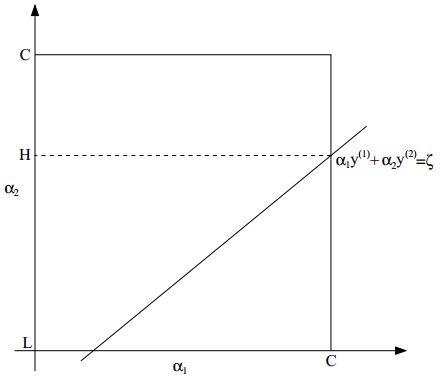
\includegraphics[scale=1]{../figures/SVM7.PNG} 
\end{center}
由约束$0\leq\alpha_i\leq C,i=1,\cdots,m$,我们可知$\alpha_1$和$\alpha_2$必须被限制在$[0,C]\times[0,C]$的框中。直线为$\alpha_1\sample{y}{1}+\alpha_2\sample{y}{2}=\zeta$。从以上的约束可以看出$L\leq\alpha_2\leq H$,否则$(\alpha_1,\alpha_2)$无法同时满足在框中的约束和直线上的约束。

又由于
\begin{eqnarray}
\alpha_1=(\zeta-\alpha_2\sample{y}{2})\sample{y}{1}
\end{eqnarray}
因此我们可以把$W(\alpha)$写成如下的形式
\begin{eqnarray}
W(\alpha_1,\alpha_2,\cdots,\alpha_m)=W((\zeta-\alpha_2\sample{y}{2})\sample{y}{1},\alpha_2,\cdots,\alpha_m)
\end{eqnarray}
将$\alpha_3,\cdots,\alpha_m$看做是常量,我们可以将$W$看作是$\alpha_2$的二次函数。如果我们忽视框的约束,那么很容易通过对二次函数求导令其等于0来求得。我们用$\alpha_2^{new,unclipped}$来表示$\alpha_2$的结果。如果我们通过最大化$W$求得的$\alpha_2$在框的约束之外,那么我们可以在$\alpha_2^{new,unclipped}$的基础上进行修剪,让其落于$[L,H]$之间,于是可以得到如下结果
\begin{eqnarray}
\alpha_2^{new}=
\left\lbrace
\begin{aligned}
H,&\ \ if \alpha_2^{new,unclipped}>H\\
\alpha_2^{new,unclipped}&\ \ if L\leq \alpha_2^{new,unclipped} \leq H\\
L,&\ \ if \alpha_2^{new,unclipped}<L
\end{aligned}
\right.
\end{eqnarray}
最后,找到了$\alpha_2^{new}$之后,再求$\alpha_1^{new}$即可。




